\chapter{Preliminares}\label{ch:preliminares}

\epigraph{Las Matem\'aticas son la creaci\'on mas bella y poderosa del esp\'iritu humano.}{Stefan Banach}

\section{Preliminares de Machine Learning}

En esta secci\'on vamos a presentar en forma resumida el procedimiento por el cual se pasa desde un set de datos a aprender a un problema de optimizaci\'on, generalmente no convexo. De ninguna manera esta exposici\'on pretender ser exhaustiva y se basa principalmente en los excelentes trabajos de \cite{bottou:2016} y \cite{mohri:2012}.

\subsection{Procedimiento formal de machine learning.}

\subsubsection{Fundamentos} 
Nuestro objetivo es elegir una funci\'on de predicci\'on que evite la memorizaci\'on mec\'anica y, en su lugar, generalice los conceptos que se pueden aprender a partir de un conjunto dado de ejemplos. Formalmente, necesitamos encontrar una $h:\mathcal{X} \rightarrow \mathcal{Y}$ tal que, dado $x \in \mathcal{X}$, el valor $h (x)$ ofrece una predicci\'on precisa sobre el valor verdadero de salida $y$. Para hacer esto, uno debe elegir la funci\'on de predicci\'on $h$ intentando minimizar el riesgo medido sobre una familia de funciones de predicci\'on adecuadamente seleccionadas \cite{vapnik:1971}, llamadas $\mathcal{H}$.

Para formalizar esta idea, supongamos que los ejemplos se muestrean a partir de una funci\'on de distribuci\'on de probabilidad conjunta $P (x, y)$. En lugar de algo que simplemente minimiza el riesgo emp\'irico (\ref{def: Riesgo empirico}), uno debe buscar encontrar $h$ que arroje un peque\~no \textit{riesgo esperado} de clasificaciones err\'oneas sobre \textit{todas las entradas posibles}, es decir, una $h$ que minimice \ref{def: riesgo esperado}:

\begin{equation}
\label{def: Riesgo empirico}
R_n(h) = \frac{1}{n}\sum\limits_{i=1}^{n}{\mathbb{1}\left[ h(x_i) \neq y \right]}
\end{equation}

\begin{equation}
\label{def: riesgo esperado}
R(h)=\mathbb{P}\left[h(x) \neq y \right] = \mathbb{E} \left[\mathbb{1} \left[h(x) \neq y \right] \right]
\end{equation}

donde $\mathbb{P}\left[A \right]$ denota la probabilidad del evento $A$  y $\mathbb{E}\left[A \right]$ denota la esperanza de la variable aleatoria indicadora del evento $A$. Tal contexto es \textit{variacional} ya que estamos optimizando sobre un conjunto de funciones, y es \textit{estoc\'astico} ya que la funci\'on objetivo implica una esperanza.

Como en la pr\'actica no se conoce $P$ \textit{a priori}, la \'unica opci\'on posible resulta ser transformar el problema a uno que dependa \'unicamente de los ejemplos $\left\lbrace\left(x_{i},y_{i}\right)\right\rbrace^{n}_{i=1}$ utilizando la \textit{ley de los grandes n\'umeros} y teniendo en cuenta dos cuestiones principales que deben abordarse: 

\begin{itemize}
	\item C\'omo elegir la familia parametrizada de funciones de predicci\'on $\mathcal{H}$
	\item C\'omo determinar (y encontrar) la funci\'on de predicci\'on particular $h \in \mathcal{H}$ que es \'optima.
\end{itemize}

\subsubsection{Elecci\'on de una familia de funciones de predicci\'on}

La familia de funciones $\mathcal{H}$ debe determinarse teniendo en cuenta tres \textit{objetivos potencialmente competitivos}. En primer lugar, $\mathcal{H}$ debe contener funciones de predicci\'on tal que en el conjunto de entrenamiento puedan lograr un riesgo emp\'irico n\'umericamente bajo, a fin de evitar el sesgo o el ajuste inadecuado de los datos. Esto se puede lograr seleccionando una familia rica de funciones o utilizando un conocimiento a \textit{priori} para seleccionar una familia bien dirigida. En segundo lugar, la brecha entre el riesgo esperado y el riesgo emp\'irico, es decir, $R(h) - R_n(h)$, debe ser peque\~na para todo $h \in \mathcal{H}$. Por lo general, esta brecha disminuye cuando se utilizan m\'as ejemplos de entrenamiento pero, debido al potencial sobreajuste, aumenta cuando usa familias de funciones m\'as ricas. En tercer lugar, $\mathcal{H}$ debe seleccionarse de manera que se pueda resolver eficientemente el problema de optimizaci\'on correspondiente, cuya dificultad puede aumentar cuando se emplea una familia m\'as rica de funciones y/o un conjunto de entrenamiento m\'as amplio.

Nuestra observaci\'on sobre la brecha entre el riesgo esperado y el emp\'irico puede entenderse utilizando la \textit{ley de los grandes n\'umeros}. La desigualdad Hoeffding \cite{hoeffding:1962} garantiza que dado $\eta>0$ existe $N \in \N$ tal que con probabilidad de al menos $1 - \eta$, uno tiene

\begin{equation}
\abs{R(h) - R_n(h)} \leq \sqrt{\frac{1}{2n} \log\left(\frac{2}{\eta}\right)} \quad \text{para un dado } h \in \mathcal{H} \quad \forall n \geq N
\end{equation}

Esta desigualdad implica la \textit{convergencia en probabilidad} del riesgo emp\'irico y  ofrece la explicaci\'on intuitiva de que la brecha disminuye a medida que se usan m\'as ejemplos de entrenamiento. Sin embargo, esta explicaci\'on es insuficiente para nuestros prop\'ositos ya que, en el contexto del machine learning, ¡$h$ no es una funci\'on fija, sino que es la variable sobre la cual se est\'a optimizando!

Por esta raz\'on, a menudo se recurre a la \textit{ley uniforme de los grandes n\'umeros} y al concepto de la dimensi\'on Vapnik-Chervonenkis (VC) de $\mathcal{H} $, una medida de la \textit{capacidad} de dicha familia de funciones \cite{vapnik:1971}, \cite{mohri:2012}. 

\begin{figure}[h]
	\centering
	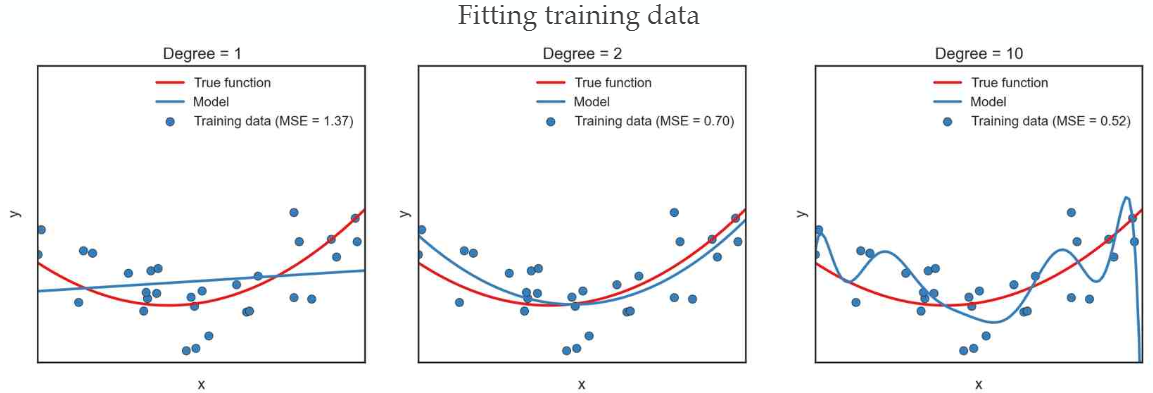
\includegraphics[scale=.3]{gfx/overfitting.png}
	\caption{Fen\'omeno de sobreajuste en polinomios de alto grado}
	\label{gfx: overfitting}
\end{figure}


Un ejemplo de \'este fen\'omeno se puede ver en la brecha entre el riesgo emp\'irico y el riesgo esperado para un conjunto de polinomios de alto grado, donde al aumentar el grado puede ser mayor ya que su alta capacidad les permite sobreajustar un conjunto dado de datos de entrenamiento. (Ver Figura \ref{gfx: overfitting})

\subsubsection{Minimizaci\'on de riesgos estructurales}

Un enfoque para elegir una funci\'on de predicci\'on que ha demostrado ser ampliamente exitoso en la pr\'actica es la \textit{minimizaci\'on del riesgo estructural} \cite{vapnik:1974}, \cite{vapnik:1998}. En lugar de elegir una familia gen\'erica de funciones de predicci\'on, sobre las cuales ser\'ia dif\'icil optimizar y estimar la brecha entre los riesgos emp\'iricos y los esperados, se elige una \textit{estructura}, es decir, una colecci\'on de familias de funciones anidadas. Por ejemplo, dicha estructura se puede formar como una colecci\'on de subconjuntos de una determinada familia $\mathcal{H}$ de la siguiente manera: dada una funci\'on de preferencia $\Omega$, se elijen varios valores de un \textit{hiperpar\'ametro} $C$, de acuerdo con cada uno de los cuales se obtiene el subconjunto $\mathcal{H}_C := \left\lbrace h \in \mathcal{H} : \Omega (h) \leq C \right\rbrace$. Dado un n\'umero fijo de ejemplos, el aumento de $C$ reduce el riesgo emp\'irico (es decir, el m\'inimo de $R_n (h) $ sobre $h \in \mathcal{H}_C$), pero, despu\'es de cierto punto, t\'ipicamente aumenta la brecha entre los riesgos esperado y emp\'irico. Este fen\'omeno se ilustra en la Figura \ref{gfx: hiperparametros}.

\begin{figure}[h]
	\centering
	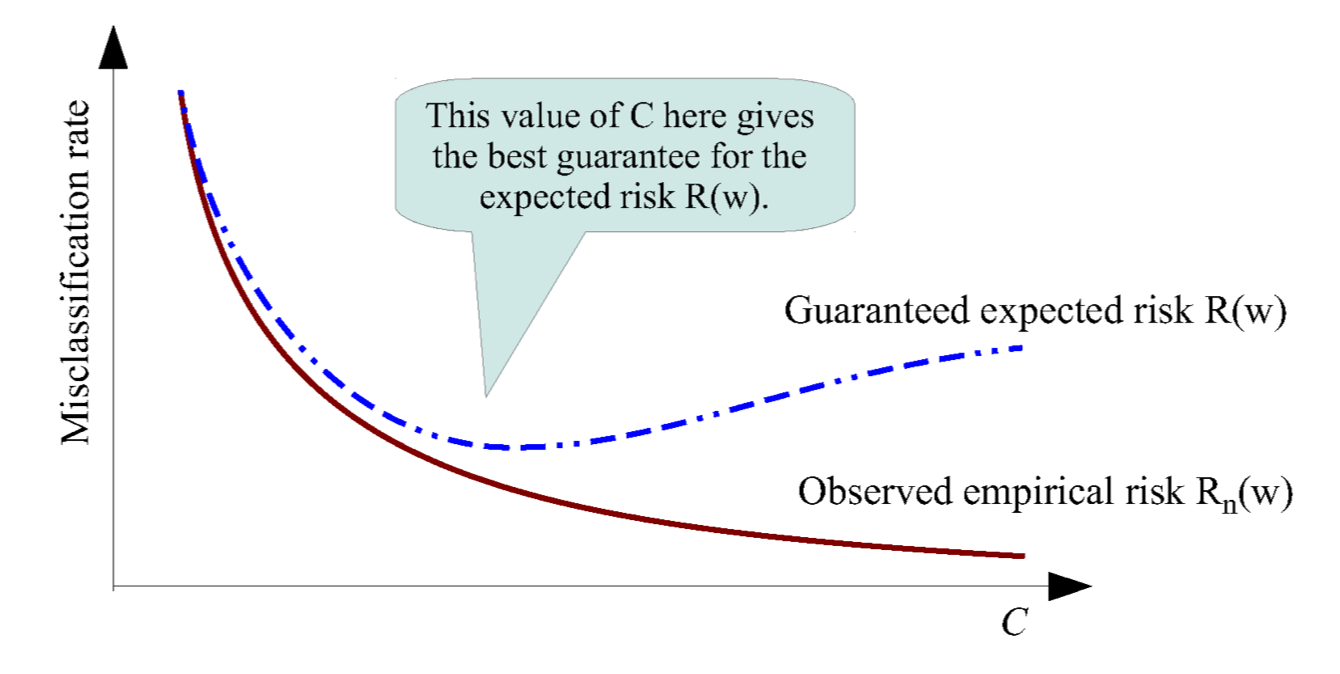
\includegraphics[scale=.3]{gfx/hyperparametros.png}
	\caption{Fen\'omeno de distancia de los riesgos en funcion de la evoluci\'on de hiperpar\'ametros}
	\label{gfx: hiperparametros}
\end{figure}

Luego, en vez de estimar la brecha entre el riesgo emp\'irico y esperado te\'oricamente, se observa que una estimaci\'on aceptable de esa brecha para el valor \'optimo de $C$ se puede obtener dividiendo los datos disponibles en tres subconjuntos.

\begin{enumerate}
	\item {\textbf{Conjunto de entrenamiento}}: Utilizado para elegir un subconjunto finito $\tilde{\mathcal{H}_C} \subset \mathcal{H}_C$ de valores que minimicen \ref{def: Riesgo empirico}
	\item{\textbf{Conjunto de validaci\'on}}: Utilizado para estimar \ref{def: riesgo esperado} sobre todo $\tilde{h} \in \tilde{\mathcal{H}_C}$ y elegir una $h_C$ \'optima
	\item{\textbf{Conjunto de prueba}}: Utilizado para estimar la brecha entre \ref{def: Riesgo empirico} y \ref{def: riesgo esperado} para la $h_C$ elegida
\end{enumerate}

Suponiendo que se ha utilizado un rango suficientemente grande para $C$, a menudo se encuentra que la mejor soluci\'on no corresponde al mayor valor de $C$ considerado; nuevamente, vea la Figura \ref{gfx: hiperparametros}.

En general, el principio de minimizaci\'on del riesgo estructural ha demostrado ser \'util para muchas aplicaciones. En lugar de codificar el conocimiento como reglas formales de clasificaci\'on, uno lo codifica mediante preferencias para ciertas funciones de predicci\'on sobre otras, luego explora el rendimiento de varias funciones de predicci\'on que se han optimizado bajo la influencia de dichas preferencias.

\subsection{Enunciados de problemas de optimizaci\'on formal}

Para continuar, debemos definir las funciones de predicci\'on y p\'erdida que aparecen en las mediciones de riesgo esperado y emp\'irico que se pretenden minimizar. 

\subsubsection{Funciones de predicci\'on y p\'erdida}
Durante esta Tesis vamos a considerar, como se mencion\'o anteriormente, que el conocimiento \textit{a priori} del problema otorga una funci\'on $h$ que parametrizaremos por un vector real $w \in \mathbb{R}^d $ sobre el cual se realizar\'a la optimizaci\'on; en vez de encarar el problema variacional. Formalmente, para un $h(\cdot ; \cdot): \mathbb{R}^{d_x} \times \mathbb{R}^d \rightarrow \mathbb{R}^{d_y}$ dado consideramos la familia de funciones de predicci\'on

\begin{equation}
\mathcal{H} := \lbrace h(\cdot ; w): w \in \mathbb{R}^d \rbrace
\end{equation}

Nuestro objetivo es encontrar la funci\'on de predicci\'on en esta familia que minimice una funci\'on de p\'erdida dada $ \ell : \mathbb{R}^{d_y} \times \mathbb{R}^{d_y} \rightarrow \mathbb{R}$. Esta mide, para un par de entrada-salida $(x, y)$, la p\'erdida $ \ell (h(x;w),y)$ cuando $h (x; w)$ e $y$ son las salidas predicha y verdadera respectivamente.

\subsubsection{Riesgo esperado}
Idealmente, el vector de par\'ametros $\omega$ se elige para minimizar la p\'erdida esperada en la que se incurrir\'ia con \textit{cualquier} par de entrada-salida. Para expresar esta idea formalmente, suponemos que las p\'erdidas se miden con respecto a una distribuci\'on de probabilidad $P (x, y)$ que representa la verdadera relaci\'on entre las entradas y las salidas. Luego, la funci\'on objetivo que deseamos minimizar es

\begin{equation}
\label{eq: Riesgo esperado}
R(w) = \int\limits_{\mathbb{R}^{d_x}\times \mathbb{R}^{d_y}} {\ell \left(h(x;w), y\right) dP(x,y)} = \mathbb{E} \left[ \ell \left( h(x;w), y \right) \right]
\end{equation}

Decimos que $R : \mathbb{R}^{d} \rightarrow \mathbb{R}$ produce el \textit{riesgo esperado} (es decir, la p\'erdida esperada) dado un vector de par\'ametro $w$ con una respectiva distribuci\'on de probabilidad $P$.

\subsubsection{Riesgo emp\'irico}
Si bien puede ser deseable minimizar (\ref{eq: Riesgo esperado}), tal objetivo es insostenible cuando no se cuenta con informaci\'on completa sobre $P$. Por lo tanto, en la pr\'actica, uno busca la soluci\'on de un problema que involucra una estimaci\'on del riesgo esperado $R_n$. En el aprendizaje supervisado, uno tiene acceso (ya sea de una vez o de manera incremental) a un conjunto de  $n \in \mathbb{N}$ muestras de entrada y salida independientes $\left\lbrace (x_i, y_i) \right\rbrace_{i=1}^{n} \subset \mathbb{R}^{d_x} \times \mathbb{R}^{d_y}$, con las cuales se puede definir la funci\'on de riesgo emp\'irico $R_n : \mathbb{R}^d \rightarrow \mathbb{R}$ dada por la ecuaci\'on 

\begin{equation}
\label{eq: Riesgo empirico}
R_n(\omega) = \frac{1}{n} \sum\limits_{i=1}^{n} {l \left( h(x;w), y\right)}
\end{equation}

En t\'erminos generales, la minimizaci\'on de $R_n$ puede considerarse el problema pr\'actico de optimizaci\'on de inter\'es. 

\subsubsection{Notaci\'on simplificada}
Para simplificar, representemos una muestra (o conjunto de muestras) por una variable aleatoria $\upxi$; por ejemplo, uno puede imaginar una realizaci\'on de $\upxi$ como una muestra \'unica $(x, y)$ de $\mathbb{R}^{d_x} \times \mathbb{R}^{d_y}$, o una realizaci\'on de $\upxi$ podr\'ia ser un conjunto de muestras $\left\lbrace(x_i, y_i)\right\rbrace_{i \in S}$. Adem\'as, podemos referirnos a la p\'erdida incurrida para un dado $(w, \upxi)$ como $F(w; \upxi )$, es decir, $F$ es la composici\'on de la funci\'on de p\'erdida y la funci\'on de predicci\'on $h$.

Para referencia futura, usamos $\upxi_{\left [ i \right ]}$ para denotar el i-\'esimo elemento de un conjunto fijo de realizaciones de una variable aleatoria $\upxi$, mientras que, comenzando en la parte \ref{pt:algoritmosestocasticos}, utilizaremos $\upxi_{\left [ k \right ]}$ para denotar el k-\'esimo elemento de una secuencia de variables aleatorias .

\subsection{Motivaci\'on para los m\'etodos estoc\'asticos}
Antes de analizar las fortalezas de los m\'etodos estoc\'asticos, como el algoritmo DE, no se debe perder de vista el hecho de que los enfoques por batch poseen algunas ventajas intr\'insecas. Primero, cuando uno ha reducido el problema estoc\'astico de minimizar el riesgo esperado $R$ para enfocarse exclusivamente en el problema determinista de minimizar el riesgo emp\'irico $R_n$, el uso de informaci\'on de gradiente completo en cada iteraci\'on abre la puerta para muchos m\'etodos de optimizaci\'on determin\'isticos. Es decir, en un enfoque por batch, uno tiene a su disposici\'on la gran cantidad de t\'ecnicas de optimizaci\'on no lineal que se han desarrollado en las \'ultimas d\'ecadas, incluido el m\'etodo de gradiente completo o gradiente de batch (\ref{algo: GD - intro}), pero tambi\'en gradiente acelerado, gradiente conjugado, cuasi-Newton y m\'etodos inexactos de Newton \cite{nocedal:2006}. Segundo, debido a la estructura de suma de $R_n$, un m\'etodo por batch puede beneficiarse f\'acilmente de la paralelizaci\'on ya que la mayor parte del c\'alculo se basa en evaluaciones de $R_n$ y $\nabla F$. Los c\'alculos de estas cantidades pueden incluso realizarse de forma distribuida.

A pesar de estas ventajas, existen razones intuitivas, pr\'acticas y te\'oricas para seguir un enfoque estoc\'astico. En pos de eso contrastaremos la iteraci\'on DE caracter\'istica (\ref{algo: DE - intro}) con la iteraci\'on de gradiente de batch completo (\ref{algo: GD - intro}).

\subsubsection{Motivación intuitiva}

En un nivel intuitivo, DE emplea información de manera más eficiente que un método por batch. Para ver esto, en una situación en la cual un conjunto de entrenamiento, not\'emoslo $S$, consta de diez copias de un conjunto de $S_{sub}$. Un minimizador de riesgo empírico para el conjunto mayor $S$ está claramente dado por un minimizador para el conjunto más pequeño $S_{sub}$, pero si se aplicara un enfoque por batch para minimizar $R_n$ sobre $S$, entonces cada iteración sería diez veces más costosa que si solo tuviese una copia de $S_{sub}$. En realidad, un conjunto de entrenamiento típicamente no consiste en duplicados exactos de datos de muestra, pero en muchas aplicaciones a gran escala los datos involucran una buena cantidad de redundancia (aproximada). Esto sugiere que usar todos los datos de muestra en cada iteración de optimización es ineficiente.

\subsubsection{Motivación práctica}

Los beneficios intuitivos que acabamos de describir se han observado repetidamente en la práctica, donde a menudo se encuentran ventajas muy reales de SG en muchas aplicaciones. Como ejemplo, la Figura \ref{gfx: de} compara el rendimiento de un método \textbf{L-BFGS} por batch\footnote[1]{El algoritmo L-BFGS no resulta importante \textit{per-se} en este trabajo, se lo menciona pues es un algoritmo de tipo batch de primer orden que resulto muy famoso en los '80 para problemas de clasificaci\'on} \cite{liu:1989} \cite{nocedal:1980} y el método SG con un incremento constante (es decir, $\alpha_k = \alpha$ para todos $k \in \N$) en un problema de clasificación binario que utiliza una función objetivo de pérdida logística y los datos del conjunto de datos RCV1 \footnote[2]{Esta colecci\'on de datos contiene caracter\'isticas de los documentos escritos originalmente en cinco idiomas diferentes y sus traducciones, en un conjunto com\'un de 6 categor\'ias, lo que lo convierte en un set de datos muy \'util a la hora de comparar algoritmos de clasificaci\'on de texto}. La figura traza el riesgo empírico $R_n$ en función del número de accesos de una muestra del conjunto de entrenamiento, es decir, el número de evaluaciones de un gradiente de muestra $\nabla f_{i_k}(w_k)$. Cada conjunto de $n$ accesos consecutivos se llama \textit{epoch}. El método por batch solo realiza un paso por \textit{epoch}, mientras que SG realiza $n$ pasos por \textit{epoch}. La trama muestra el comportamiento en los primeros 10 \textit{epochs}. La ventaja de SG es llamativa y representativa del comportamiento típico en la práctica. 

Sin embargo, se debe tener en cuenta que para obtener un comportamiento tan eficiente, era necesario ejecutar SG varias veces usando diferentes opciones para $\alpha$ hasta que se identificara una buena opción para este problema en particular. Discutimos cuestiones teóricas y prácticas relacionadas con la elección de incrementos en nuestro análisis en la parte \ref{pt:algoritmosestocasticos}.


\begin{figure}[h]
	\centering
	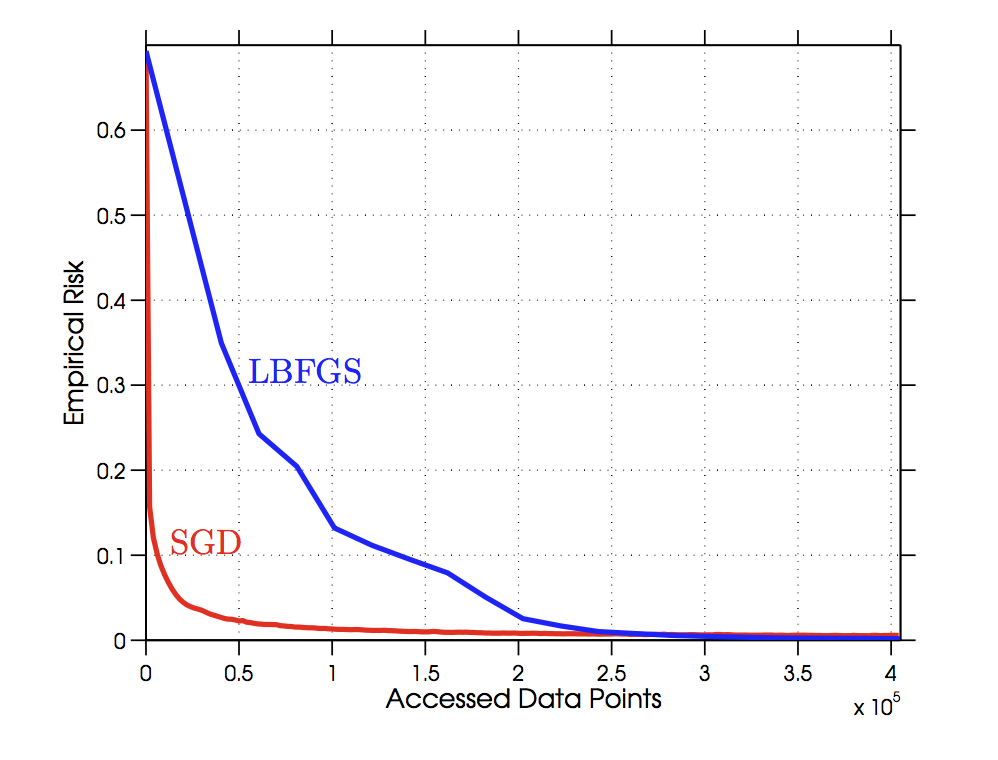
\includegraphics[scale=.3]{gfx/de.png}
	\caption{Riesgo empírico $R_n$ en función del número de puntos de datos accedidos (ADP) para un método \textbf{L-BFGS} por batch y el método de gradiente estocástico (SG) en un problema de clasificación binaria con un objetivo de pérdida logística y el conjunto de datos RCV1. SG se ejecutó con un incremento fijo de $\alpha  = 4$}
	\label{gfx: de}
\end{figure}

\subsubsection{Motivación Teórica }

También se pueden citar argumentos teóricos para una preferencia de DE sobre un enfoque por batch. Ahora vamos a dar un peque\~no resumen de estos argumentos, que se estudian con m\'as profundidad y m\'as detalle en la parte \ref{pt:algoritmosestocasticos}:

\begin{itemize}
	\item Es bien sabido que un enfoque por batch puede minimizar $R_n$ a un ritmo r\'apido. Por ejemplo, si $R_n$ es fuertemente convexo (ver \ref{def: Fuertemente convexa}) y uno aplica un m\'etodo de descenso de gradiente por batch, entonces existe una constante $\rho \in (0,1)$ tal que, para todo $k \in \N$, el error de entrenamiento satisface:
	
	\begin{equation}
	\label{Complejidad riesgo en batch}
	R_n(w_k) - R_n^* \leq \mathcal{O} \left(\rho^k\right)
	\end{equation}
	
	Donde $R_n^*$ denota el valor m\'inimo de $R_n$. La velocidad de convergencia exhibida aquí se conoce como \textit{convergencia lineal} en la bibliograf\'ia de optimización \cite{ortega:2000} y \textit{convergencia geométrica} en la comunidad de investigación de machine learning; simplemente nos referiremos a él como convergencia lineal. De (\ref{Complejidad riesgo en batch}), se puede concluir que, en el peor de los casos, el número total de iteraciones en las que el error de entrenamiento puede estar por encima de un valor dado de $\epsilon >0$ es proporcional a $\log \left(\frac{1}{\epsilon}\right)$. Esto significa que, con un costo por iteración proporcional a $n$ (debido a la necesidad de calcular $\nabla F(w_k)$ para todo $k \in \N$), el trabajo total requerido para obtener $\epsilon-$optimalidad para un método de gradiente por batch es proporcional a $n \log\left(\frac{1}{\epsilon}\right)$.
	
	\item La velocidad de convergencia de un método estocástico básico es más lenta que para un método de gradiente por batch; por ejemplo, si $R_n$ es estrictamente convexo y cada $i_k$ se muestrea uniformemente desde en $\sett{1, \dots, n}$, entonces, para todo $k \in \N$, las iteraciones DE satisfacen la propiedad de convergencia sublineal (ver \ref{theorem: DE en fuertemente convexo y alfa decreciente converge en l1}):
	
	\begin{equation}
	\label{Complejidad riesgo en de}
	\expectation{R_n(w_k) - R_n^*} = \mathcal{O} \left(\frac{1}{k}\right)
	\end{equation}
	
	Sin embargo, es cr\'itico notar que ni el costo de iteración ni el orden dependen del tamaño del conjunto de muestras $n$. Esto significa que el trabajo total requerido para obtener $\epsilon-$optimalidad para DE es proporcional a $\frac{1}{\epsilon}$. Es cierto que esto puede ser mayor que $n \log \left(\frac{1}{\epsilon}\right)$ para valores chicos de $n$ y $\epsilon$, pero la comparación favorece a DE cuando se pasa al régimen de \textit{big data} donde $n$ es grande y uno se encuentra limitado \'unicamente por un presupuesto de tiempo computacional.
	
	\item Otra característica importante de DE es que produce la misma velocidad de convergencia que en (\ref{Complejidad riesgo en de}) para el error en el riesgo esperado, $R - R^**$, donde $R^*$ es el valor mínimo de $R$. Específicamente, aplicando la iteración DE, pero con $g(wk, \upxi_{k})$ reemplazado por $\nabla f (w_k; \upxi_{k})$ con cada $\upxi_{k}$ tomado independientemente de acuerdo con la distribución P, vale:
	
	\begin{equation}
	\expectation{R(w_k) - R^*} = \mathcal{O} \left(\frac{1}{k}\right)
	\end{equation}
	
	Que nuevamente es una velocidad sublineal pero en el riesgo esperado, algo que es imposible estimar en los m\'etodos de batch. Por lo tanto, deducimos que en el regimen de \textit{big data} minimizar el riesgo emp\'irico o el riesgo esperado es equivalente, lo que potencia la generalidad de las soluciones halladas por DE.
	
\end{itemize}

En resumen, existen argumentos intuitivos, prácticos y teóricos a favor de enfoques estocásticos sobre m\'etodos por batch en optimización para el machine learning a gran escala. Sin embargo, no pretendemos que los métodos por batch no tengan lugar en la práctica; por ejemplo si en la Figura \ref{gfx: de} se considerara un mayor número de \textit{epochs}, entonces se vería que el algoritmo de batch eventualmente mejora al método estocástico y produce un menor error de entrenamiento. Esto motiva que muchos métodos propuestos recientemente intenten combinar las mejores propiedades de los algoritmos por batch y estocásticos. Además, la iteración de DE es difícil de paralelizar y requiere una comunicación excesiva entre nodos en una configuración de computación distribuida, proporcionando un mayor impulso para el diseño de algoritmos de optimización nuevos y mejorados. \cite{agarwal:2017} \cite{atchade:2014}

\section{Preliminares Matem\'aticos}

\subsection{Espectro}

\begin{definition}
	Sea $f : X \rightarrow Y$, con $X,Y$ Banach, $f \in L(X,Y)$; definimos el espectro de $f$ de la siguiente manera:
	
	\begin{equation*}
		\sigma(f) = \sett{\alpha \in \C \tq f- \alpha \text{ no es inversible}}
	\end{equation*}
	
	Si este conjunto fuese vac\'io, entonces $R_{\lambda} = \left(\lambda -f\right)^{-1}$ ser\'ia holomorfa en $\C$ y no constante, absurdo por Liouville. Luego, como es no vac\'io existe el supremo pues $\C$ es completo; al supremo del espectro le decimos radio espectral:
	
	\begin{equation*}
	\rho(f) = \sup \sett{\abs{\alpha} \tq \alpha \in \sigma(f)}
	\end{equation*}
	
\end{definition}

\begin{proposition}
	\label{prop: teorema de gelfand}
	Sea $f \in L(X,Y)$ un operador lineal, entonces:
	
	\begin{equation*}
		\rho(f) = \lim\limits_{n \to \infty} \norm{f^n}^{\frac{1}{n}}
	\end{equation*}
	
\end{proposition}

\begin{theorem}[Teorema espectral para operadores compactos autoadjuntos]
	Sea $X$ Hilbert y $T \in L(X)$ compacto y autoadjunto, entonces $T$ admite numerables autovalores distintos. 
	
	Es m\'as si $\sett{\lambda_1, \dots, \lambda_n, \dots} \subset \sigma_p(T) \cap \R^{\ast}$ y $P_n = P_{\ker(T-\lambda_n)}$ (donde notamos $P_{\ker(T-\lambda_n)}$ a la proyecci\'on ortogonal con respecto al autoespacio de $T$ asociado al autovalor $\lambda_n$) luego $P_nP_n = P_nP_m = 0$ si $n \neq m$ y vale:
	
	\begin{equation}
	\label{eq: Teorema espectral}
	T = \Bigsum{n \in \N}{\lambda_n P_n}
	\end{equation}
\end{theorem}

\begin{proposition}
	\label{prop: calculo funcional}
	
	Sea $f \in L(X,Y)$ un operador compacto autoadjunto y $h$ una funci\'on holomorfa en un entorno $U \subset \C$ con $\sigma(f) \subset U$, entonces:
	
	\begin{equation*}
		\sigma \left(h(f)\right) = h(\sigma(f))
	\end{equation*}
	
	Donde definimos $h(f) = \Bigsum{n \in \N}{h(\lambda_n) P_n} \in L(X,Y)$ pues $f$ es compacto.
	
\end{proposition}

\begin{corollary}
	Sea $A \in \C^{n \times n}$ una matriz diagonalizable con autovalores $\sett{\lambda_1, \dots, \lambda_n}$ y $f \in \C_n[X]$ un polinomio con coeficiente complejos de grado $n$, entonces $f(A)$ tiene autovalores $\sett{f(\lambda_1), \dots, f(\lambda_n)}$.
\end{corollary}

\subsection{Variedades diferenciables y Teorema de la variedad estable}

Cuando estudiemos los algoritmos de tipo batch es habitual analizar el algoritmo como $x_{k+1} \gets g(x_k)$ para una $g : X \rightarrow X$ inducida; o sea uno analiza las \'orbitas bajo la acci\'on de $g$ en una variedad dada $X$. Con esa motivaci\'on repasemos los conceptos b\'asicos de sistemas din\'amicos.

\subsubsection{Un repaso de Variedades}

\begin{definition}{[Cap\'itulo 1 de \cite{lee:00}]}
	Dado un espacio topol\'ogico $X$ decimos que es una variedad diferenciable de dimensi\'on $d$ si:
	
	\begin{itemize}
		\item $X$ es Haussdorf
		\item Para todo cubrimiento por abiertos de $X$ existe un subcubrimiento numerable
		\item Existe un atlas suave para $X$, o sea existe un conjunto de pares $\sett{\left(U_i, \phi_i\right)}$ tales que:
		
		\begin{enumerate}
			\item Para todo $x \in X$ existe $(U,\phi)$ con $x \in U$ y $\phi: U \rightarrow \phi{U}$ homeomorfismo
			\item Si existen dos cartas $(U,\phi), (V,\psi)$ en el entorno de $x$ con $U \cap V \neq \emptyset$ entonces $\phi \circ \psi^{-1} : \psi(U\cap V )\rightarrow \phi(U\cap V)$ es difeomorfismo
		\end{enumerate}
	\end{itemize}
	
\end{definition}

\begin{definition}{[Cap\'itulo 6 de \cite{lee:00}]}
	Dada una variedad de dimensi\'on $d$ que notaremos como $\mani$ y el espacio de medida $\left(\R^d, \mathcal{B}, \mu\right)$, decimos que $E \subset \mani$ tiene \textit{medida cero} si existe un atlas $\mathcal{A} = \sett{U_i, \phi^i}_{i \in \N}$ tal que $\mu \left(\phi^i \left(E \cap U_i \right) \right) = 0$ para todo $i$. En este caso usamos el abuso de notaci\'on $\mu(E) = 0$.
\end{definition}

\begin{definition}{[Cap\'itulo 3 de \cite{lee:00}]}
	El diferencial de $g$ es un operador lineal $D_g(x): \mathcal{T}_x \mapsto \mathcal{T}_{g (x)}$, donde $\mathcal{T}_x$ es el espacio tangente de $X$ en el punto $x$. Dada una curva $\gamma$
	en $X$ con $\gamma(0) = x$ y $d\gamma(0) = v \in \mathcal{T}_x$, el operador lineal se define como $D_g(x)v = \dfrac{d (g\circ \gamma)}{dt}(0) \in T_{g (x)}.$ El determinante del operador lineal $det (D_g (x))$ es el determinante de la matriz que representa $D_g (x)$ con respecto a una base arbitraria y resulta invariante por cambios de base.
\end{definition}

\begin{proposition}
	Sea $X$ una variedad de dimensi\'on $d$, luego para todo $x \in X$ vale que $\mathcal{T}_x$ es un espacio vectorial de dimensi\'on $d$.
\end{proposition}

\begin{theorem}
	\label{theorem: Teorema de la funcion inversa}
	Sea $F: X \mapsto N$ una funci\'on diferenciable tal que $dF_x$ es un isomorfismo lineal, luego existe $x \in U \subset X$ abierto tal que $F \vert_U$ es un difeomorfismo; es decir que $F, F^{-1} \in C^{\infty}(U)$.
\end{theorem}

\begin{proposition}
	\label{prop: Localmente Lipschitz preserva medida}
	Sea $f : \R^d \rightarrow \R^d$ una funcion localmente Lipschitz, luego si $\mu(E) = 0$ vale que $\mu(f(E)) = 0$
\end{proposition}

\begin{lemma}
	\label{Difeomorfismos locales preservan medida cero}
	Sea $E \subset \mani$ tal que $\mu(E) = 0$; si $\det \left(Dg(x)\right) \neq 0$ para todo $x \in \mani$, luego $\mu\left(g^{-1}(E)\right) = 0$
\end{lemma}

\begin{proof}
	Sea $h = g^{-1}$ y $\left(V_i, \psi^i\right)$ una colecci\'on de cartas en el dominio de $g$, si verificamos que $\mu\left(h\left(E\right) \cap V_i\right) = 0$ para todo $i \in \N$ entonces:
	
	\begin{equation*}
	\mu(h(E)) = \mu \left(\Bigcup{i \in \N}{h(E) \cap V_i}\right) \le \Bigsum{i \in \N} \mu \left(h(E) \cap V_i\right) = 0
	\end{equation*}
	
	Sin p\'erdida de generalidad podemos asumir que $h(E) \subseteq V$ con $(V, \psi) \in \sett{(V_i, \phi^i)}$ una carta determinada. Sea $\mathcal{A} := \sett{\left(U_i, \varphi^i \right)}$ un atlas de $\mani$ y notemos $E_i = E \cap U_i$; luego $E = \Bigcup{i \in \N}{E_i} = \Bigcup{i \in \N}{{\varphi^i}^{-1} \circ \varphi^{i} \left(E_i\right)}$ por lo que:
	
	\begin{equation*}
	\begin{aligned}
	\mu\left(\psi \circ h(E)\right) & = & \mu \left(\psi \circ h \left(\Bigcup{i \in \N}{{\varphi^i}^{-1} \circ \varphi^{i} \left(E_i\right)}\right)\right)\\
	& \le & \Bigsum{i \in \N}{\mu \left(\psi \circ h \circ {\varphi^{i}}^{-1} \left(\varphi^i (E_i)\right)\right)}
	\end{aligned}
	\end{equation*}
	
	Por hip\'otesis $\varphi^i(E_i)$ es de medida cero, luego como $g$ es difeomorfismo local por \ref{theorem: Teorema de la funcion inversa}  entonces $\psi \circ h \circ {\varphi^{i}}^{-1} \in C^1$. Como $f \in C^1(\R^d)$ implica que es localmente Lipschitz concluimos por \ref{prop: Localmente Lipschitz preserva medida} que ${\mu \left(\psi \circ h \circ {\varphi^{i}}^{-1} \left(\varphi^i (E_i)\right)\right)} = 0$ para todo $i \in \N$. \qed
	
\end{proof}

Finalizamos con un resultado natural, pero no por eso menos crucial a la hora de analizar la probabilidad de un conjunto dado en $X$.

\begin{proposition}
	\label{prop: Dimension menor tiene medida 0}
	Sea $N \inc M$ una subvariedad de dimensi\'on $n < m$, luego para todo $U \subset N$ abierto relativo vale que $\mu(U) = 0$
\end{proposition}

\subsubsection{Teorema de la variedad estable}

\begin{definition}
	Sea $f : \R^d \rightarrow \R$ tal que $f \in C^2$, (notando $\nabla^2 f (x) = \text{Hessiano de } f \text{ evaluado en } x$) y $x^* \in \R^d$, luego:
	
	\begin{itemize}
		\item Decimos que $x^*$ es punto cr\'itico de $f$  si $\nabla f(x^*) = 0$
		\item Decimos que $x^*$ es un m\'inimo local de $f$ si es un punto cr\'itico y $\lambda_{min} \left(\nabla ^2 f(x^*)\right) > 0$
		\item Decimos que $x^*$ es un punto silla estricto de $f$ si es un punto cr\'itico y $\lambda_{min} \left(\nabla ^2 f(x^*)\right) < 0$ 
	\end{itemize}
	
	Notaremos $\mani^*$ al conjunto de puntos silla estrictos de $f$.
	
\end{definition}

\begin{theorem}
	\label{teo: variedad local estable central}
	Sea $x^*$ un punto fijo de $g \in C^{r}(\mani)$ un difeomorfismo local. Supongamos que $E = E_s \oplus E_u$ donde 
	
	\begin{equation*}
	\begin{aligned}
	E_s & = & \langle \sett{v_i \ / \ Dg(x^*)v_i = \lambda_i v_i \quad , \quad \lambda_i \le 1} \rangle \\
	E_u & = & \langle \sett{v_i \ / \ Dg(x^*)v_i = \lambda_i v_i \quad , \quad \lambda_i > 1} \rangle \\
	\end{aligned}
	\end{equation*}
	Entonces existe $W_{loc}^{cs} \inc \mani$ una inyecci\'on difeomorfa local tangente a $E_s$ en $x^*$ llamado la \textit{variedad local estable central} que cumple que existe $B \ni x^*$ entorno tal que $g\left(W_{loc}^{cs}\right) \cap B \subseteq W_{loc}^{cs}$ y $\Bigcap{k \in \N}{g^{-k}(B)} \subseteq W_{loc}^{cs}$
\end{theorem}

\begin{proof}
	Ver Teorema III.1 de \cite{schub:1987}
\end{proof}

\subsection{Procesos Estoc\'asticos}

Debido a la naturaleza de los algoritmos estoc\'asticos, tiene sentido repasar los conceptos b\'asicos que utilizaremos en su estudio.

\subsubsection{Esperanza condicional}

Dado un espacio de probabilidad $\left(\Omega, \mathcal{F}, P\right)$ definimos una \textit{variable aleatoria } como una funci\'on $X : \Omega \mapsto \R$ tal que $X^{-1}(B) \in \mathcal{F}$ para todo $\B \in \mathcal{B}$ boreliano.

Por otro lado, dado un conjunto $\Omega$ y una familia $\left(X_{\gamma}\right)_{\gamma \in C}$ tal que $X_{\gamma}: \Omega \mapsto \R$ definimos la \textit{$\sigma$ algebra generada por las $X_\gamma$} $\mathcal{F} = \sigma\left(\sett{X_{\gamma}}\right)$ como la menor $\sigma$ \'algebra (en el sentido de la inclusi\'on) tal que todas las $X_{\gamma}$ son $\mathcal{F}$ medibles.

Recordemos adem\'as:

\begin{theorem}[Teorema de la convergencia mon\'otona]
	\label{theorem: Convergencia monotona}
	Sea $(f_n)$ una sucesi\'on positiva de elementos medibles en $(\Omega, \Sigma, \mu)$ un espacio de medida tal que $f_n \nearrow f$; luego:
	
	\begin{equation*}
		\int\limits_{\Omega} {f_n d\mu} \nearrow \int\limits_{\Omega}{f d\mu} 
	\end{equation*} 
\end{theorem}

\begin{theorem}[Teorema de la convergencia dominada]
	\label{theorem: Convergencia dominada}
	Sea $(f_n)$ una sucesi\'on de elementos medibles en $(\Omega, \Sigma, \mu)$ un espacio de medida tal que $f_n \rightarrow f$ ctp; si existe $g \in L^1$ tal que $\abs{f_n} \leq g$ entonces:
	
	\begin{equation*}
	\int\limits_{\Omega} {\abs{f_n -f}d\mu} \rightarrow 0
	\end{equation*} 
\end{theorem}

\begin{remark}
	Una observaci\'on clave en el an\'alisis de los algoritmos de tipo estoc\'astico es que si llamamos ${W} := \sett{w_k}$ a las iteraciones del algoritmo, entonces notemos que podemos ver a $w_k$ como una variable aleatoria. En efecto, $w_k := w_{k-1} - \alpha_k g(w_k, .) : \Omega \rightarrow \R$ y por hip\'otesis es $\F$ medible; es m\'as, podemos ver a $W : \N_+ \times \Omega \rightarrow \R$ dado por $W(k, \omega) := w_k$ como un proceso estoc\'astico discreto.
\end{remark}

\begin{proposition}
	\label{def: esperanza condicional}
	Sea $\left(\Omega, \F, P\right)$ un espacio de probabilidad y $X$ una variable aleatoria tal que $X \in L^1(\Omega)$ ( es decir $\expectation{\abs{X}} < \infty$). Si $\mathcal{G}$ es una sub-$\sigma-$algebra de $\F$ entonces existe $Y$ variable aleatoria tal que:
	
	\begin{enumerate}
		\item $Y$ es $\mathcal{G}$ medible
		\item $Y \in L^1(\Omega)$
		\item Para todo $G \in \mathcal{G}$ vale:
		
		\begin{equation*}
			\int\limits_{G} {Y dP} = \int\limits_{G} {X dP}
		\end{equation*}
	\end{enumerate}

	Es m\'as, si $\widetilde{Y}$ es otra variable aleatoria que cumple las propiedades, entonces $Y = \widetilde{Y}$ ctp.
	
\end{proposition}

\begin{definition}
	Dados $X,\mathcal{G}$ como en la proposici\'on, a la variable aleatoria cuya existencia se prueba en \ref{def: esperanza condicional} se llama \textit{una versi\'on de la esperanza condicional de $X$ dado $\mathcal{G}$} y se lo nota $\expectation{X \vert \mathcal{G}}$.
	
	A su vez, dada $Z$ otra variable aleatoria definimos la \textit{esperanza condicional de $X$ dado $Z$} como $\expectation{X \vert Z} := \expectation{X \vert \sigma(Z)}$
	
\end{definition}

\begin{proof}
	Demostremos la existencia y unicidad:
	
	\begin{enumerate}
		\item {\textbf{Unicidad ctp}}
		
		Sea $X \in L^1$ e $Y,\widetilde{Y}$ dos versiones de $\expectation{X \vert \mathcal{G}}$ tal que no son iguales ctp, luego como $\sett{Y - \widetilde{Y} > \frac{1}{n}} \nearrow \sett{Y > \widetilde{Y}}$ existe $N$ tal que:
		
		\begin{equation*}
			P\left(Y - \widetilde{Y} > \frac{1}{N}\right) > 0
		\end{equation*}
		
		Luego como $Y, \widetilde{Y}$ son $\mathcal{G}$ medibles $\sett{Y - \widetilde{Y} > \frac{1}{N}} \in \mathcal{G}$ y entonces:
		
		\begin{equation*}
			0 \underbrace{=}_{Y,\widetilde{Y} = \expectation{X \vert \mathcal{G}}} \int\limits_{\sett{Y - \widetilde{Y} > \frac{1}{N}}} {Y - \widetilde{Y}} \geq \frac{1}{N} P \left(\sett{Y - \widetilde{Y} > \frac{1}{N}}\right) > 0
		\end{equation*}
		
		Luego $Y = \widetilde{Y}$ ctp.
		
		\item {\textbf{Existencia en $L^2$}}
		
		Sea $\mathcal{K} = L^2(\Omega, \mathcal{G}, P)$, sabemos que $\mathcal{K} $ es completo en $L^2(\Omega, \mathcal{F}, P)$ y como $L^2$ es Hilbert existe $Y \in \mathcal{K} $ tal que:
		
		\begin{equation*}
			\expectation{\left(X - Y \right)^2} = \inf \sett{\expectation{\left(X - W \right)^2} \tq W \in \mathcal{K}}
		\end{equation*}
		
		\begin{equation*}
			\ip{X-Y, Z} = 0 \quad Z \in \mathcal{K}
		\end{equation*}
		
		Luego si $G \in \mathcal{G}$ entonces $Z = 1_{G} \in \mathcal{G}$ por lo que:
		
		\begin{equation*}
			\ip{X-Y, 1_G} = 0 \Longrightarrow \ \int\limits_{G} {XdP} = \int\limits_{G}{Y dP}
		\end{equation*}
		
		Concluimos que $Y = \expectation{X \vert \mathcal{G}}$
		
		\item {\textbf{Existencia en $L^1$}}		
		
		Notemos que basta verlo para $X \geq 0$, luego existen $X_n \geq 0$ acotadas tal que $X_n \nearrow X$; como cada $X_n \in L^2$ si definimos $Y = \limsup \expectation{X_n \vert \mathcal{G}}$ entonces \ref{theorem: Convergencia monotona} demuestra lo que necesitabamos.\qed
		
	\end{enumerate}
	
\end{proof}

\begin{theorem}[Propiedades de la esperanza condicional]
	\label{theorem: Propiedades de esperanza condicional}
	Sea $\left(\Omega, \mathcal{F}, P\right)$ un espacio de medida, $X \in L^1$ y $\mathcal{G}, \mathcal{H}$ sub-$\sigma-$\'algebras de $\F$, luego:
	
	\begin{enumerate}
		\item $\expectation{\expectation{X \vert \mathcal{G}}} = \expectation{X}$
		\item Si $X$ es $\mathcal{G}$ medible entonces $X = \conditionalExpectation{X}{\G} $ ctp
		\item $\conditionalExpectation{aX + bY}{\G} = a\conditionalExpectation{X}{\G} + b \conditionalExpectation{Y}{\G}$
		\item Si $X \geq 0$ ctp, entonces $\conditionalExpectation{X}{\G} \geq 0$ ctp
		\item Si $0 \leq X_n \nearrow X$ entonces $\conditionalExpectation{X_n}{\G} \nearrow \conditionalExpectation{X}{\G}$
		\item Si $0 \leq X_n$ ctp entonces $\conditionalExpectation{\liminf X_n}{\G} \leq \liminf \conditionalExpectation{X_n}{\G}$
		\item Si $\abs{X_n} \leq V$ con $V \in L^1$ entonces si $X_n \rightarrow X$ ctp vale que $\conditionalExpectation{X_n}{\G} \rightarrow \conditionalExpectation{X}{G}$ ctp.
		\item Si $\mathcal{H}$ es una sub-$\sigma-$\'algebra de $\G$ entonces:
		
		\begin{equation*}
			\conditionalExpectation{X}{\G \vert \mathcal{H}} := \conditionalExpectation{\conditionalExpectation{X}{\G}}{\mathcal{H}} = \conditionalExpectation{X}{\mathcal{H}}
		\end{equation*}
		
		\item Si $Z$ es $\G$ medible y acotada entonces $\conditionalExpectation{ZX}{\G} = Z \conditionalExpectation{X}{\G}$ ctp
		\item Si $\mathcal{H}$ es independiente de $\sigma\left(\sigma(X), \G\right)$ entonces:
		
		\begin{equation*}
			\conditionalExpectation{X}{\sigma \left(\G, \mathcal{H}\right)} = \conditionalExpectation{X}{G} \ ctp
		\end{equation*}
		
		En particular, si $X$ es independiente de $\G$ vale que $\conditionalExpectation{X}{\G} = \expectation{X}$ ctp. 
		
	\end{enumerate}
	
\end{theorem}

\begin{proof}
	Una buena referencia resulta \cite{williams:1991}. No se incluye la demostraci\'on por su extensi\'on y porque no resulta crucial al presente trabajo.
\end{proof}

\subsubsection{Martingalas y Cuasi-martingalas}

\begin{definition}
	Dada una sucesi\'on creciente (en el sentido de la inclusi\'on) de $\sigma$ \'algebras $\F_n \subset \F$ decimos que $\sett{\F_n}$ es una \textit{filtraci\'on} y que el espacio $\left(\Omega, \F, \sett{F_n}, P\right)$ es un espacio filtrado.
	
	Un proceso $X  = \left(X_n\right)$ decimos que es adaptado si $X_n $ es $\F_n$ medible para todo $n$ en un espacio filtrado.
	
	A su vez, dado un proceso $\left(X_n\right)$, \'este induce una filtraci\'on (llamada natural) en un espacio de probabilidad $\left(\Omega, \F, P\right)$ dada por $\F_n = \sigma\left(X_1, \dots, X_n \right)$
	
\end{definition}

\begin{definition}
	Dado un espacio filtrado, decimos que un proceso $X = \left(X_n\right)$ es una martingala relativa a la filtraci\'on $\sett{\F_n}$ si:
	
	\begin{itemize}
		\item $X$ es adaptado
		\item $X_n \in L^1$
		\item $\conditionalExpectation{X_n}{\F_{n-1}} = X_{n-1}$ ctp
	\end{itemize}

	A su vez decimos que es una (sub)supermartingala si vale la condici\'on $\conditionalExpectation{X_n}{\F_{n-1}} (\leq)\geq X_{n-1}$
	
\end{definition}

\begin{definition}
	Dado un espacio filtrado y $X$ un proceso integrable y adaptado, decimos que es una \textit{cuasi-martingala} si para todo $n \in \N$:
	
	\begin{equation}
		\mathbb{Var}_n(X) = \sup\limits_{J \subset \sett{1, \dots, n}} \sett{\expectation{\sum\limits_{\substack{i_k \in J \\ 1 \leq k \leq \abs{J}}}{\abs{\conditionalExpectation{X_{i_{k+1}} - X_{i_k}}{\F_{i_{k}}}}}}} < \infty
	\end{equation}
	
\end{definition}

\begin{remark}
	El concepto de cuasi-martingalas es una generalizaci\'on natural de las martingalas, submartingalas y supermartingalas. Fueron introducidos por primera vez por Fisk \cite{fisk:1965} para extender la descomposici\'on de Doob-Meyer a una clase m\'as grande de procesos. La forma en que las cuasimartingalas se relacionan con sub y s\'uper martingalas es muy similar a c\'omo las funciones de variaci\'on acotada se relacionan con funciones crecientes y decrecientes. En particular, mediante la descomposici\'on de Jordan, cualquier funci\'on de variaci\'on acotada en un intervalo se descompone como la suma de una funci\'on creciente y una funci\'on decreciente. De manera similar, un proceso estoc\'astico es una cuasimartingala si y solo si puede escribirse como la suma de una submartingala y una supermartingala. Este importante resultado fue mostrado primero por Rao \cite{rao:1969}, y signific\'o el inicio de la extensi\'on de gran parte de la teor\'ia de submartingalas  a cuasimartingalas.
\end{remark}

\begin{proposition}
	Toda martingala, submartingala o supermartingala es una cuasi-martingala
\end{proposition}

\begin{proof}
	En efecto, reemplazando $X$ por $-X$ podemos suponer que $\conditionalExpectation{X_{i_{k+1}} - X_{i_k}}{\F_{i_k}} \geq 0$, luego por \ref{theorem: Propiedades de esperanza condicional} resulta que $\mathbb{Var}_n(X) = \abs{\expectation{X_n - X_0}} < \infty$. \qed
\end{proof}

Ahora estamos en condiciones de enunciar el resultado principal de esta secci\'on: \textbf{El teorema de convergencia de cuasi-martingalas}. Este resultado es crucial en el an\'alisis de convergencia de algoritmos estoc\'asticos porque veremos m\'as adelante que el proceso estoc\'astico $\sett{w_k}$ inducido por el algoritmo induce una cuasi-martingala $\sett{w_k'}$ que ser\'a convergente; de lo cual deduciremos la convergencia de $\sett{w_k}$.

\begin{definition}
	\label{def: Variaciones positivas de un proceso}
	Dado un proceso estoc\'astico $\sett{u_k}$ adaptado a un espacio filtrado $\left(\Omega, \F, \sett{\mathcal{P}_k}, P\right)$ definimos el \textit{proceso de variaciones positivas} asociadas a $\sett{u_k}$ como :
	
	\begin{equation}
	\delta^u_k := \left\lbrace \begin{array}{cc}
	1 & \text{ si } \expectationfilt{u_{k+1} - u_k} > 0 \\
	0 & \text{ si no }
	\end{array}\right.
	\end{equation}
	
\end{definition}

\begin{theorem}[Teorema de convergencia de cuasi-martingalas]
	\label{theorem: Convergencia de cuasi martingalas}
	Dado un proceso estoc\'astico $\sett{u_k}$ adaptado a un espacio filtrado $\left(\Omega, \F, \sett{\mathcal{P}_k}, P\right)$ tal que:
	
	\begin{itemize}
		\item $u_k \geq 0$ ctp
		\item $\sum\limits_{k=1}^{\infty} {\expectation{\delta^u_k\left(u_{k+1} - u_k\right)}} < \infty$
	\end{itemize}
	
	Entonces $\sett{u_k}$ es una cuasi-martingala tal que $u_k \rightarrow u_{\infty} \geq 0$ ctp.
	
\end{theorem}

\begin{proof}
	Una buena revisi\'on de la demostraci\'on se encuentra en el cap\'itulo 9 de \cite{metivier:1983}
\end{proof}
